% !TEX root = ../thesis.tex
%\chapter{[Core contribution]: Approach}
\chapter{Experiments}
\label{capitolo4}
\thispagestyle{empty}

\iffalse

This is the chapter where you explain how you approach the problem and how you intend to meet the requirements identified in the previous chapter. In short, here you explain your \emph{solution}. But attention: you won't be able to describe every aspect of your thesis project here, in one single chapter. You will need more than one for that. So, this is the chapter where you explain your solution in terms of the general approach and the design decisions that you make:

\begin{itemize}
\item[\Square] Identify the target \emph{actors} that will benefit from your solution, describe them.
\end{itemize}

\fi


\section{Our Societal Focus: Gender Gap}
Modern societies, as well as every society in human history, are faced with various and different social problems (i.e. conditions or behaviors that have negative consequences for large numbers of people and that are generally recognized as conditions or behaviors that need to be addressed). Global climate change, overpopulation, poverty and homelessness, or racial discrimination are just a few examples -- the tip of the iceberg -- but many more social problems exist and are far from being resolved. For the purpose of our research, we decided to focus on discrimination problems, and in particular on the so called ``\textbf{gender gap}''. According to \cite{cambridge2013gender}, gender gap is definable as:
\begin{quote}\emph{A difference between the way men and women are treated in society, or between what men and women do and achieve.} \cite{cambridge2013gender}\end{quote}
Specifically, the focus of our experiments is \textit{gender pay gap}, already mentioned in Section~\ref{section:the_glassdoor_method}, that is, the average difference between the remuneration for men and women in the workforce, or, in other words, a measure of what women are paid relative to men. The experiments are centered on the economical perspective because it is the easiest to measure in the data, being quantifiable for example as a number representative of a person's average monthly salary, but other facets of the gender gap problem will come into play when dealing with sociological studies.


\section{Datasets Description}
The main purpose of this research is to combine the technological perspective with the sociological one, in order to analyze the strenghts and weaknesses of the adopted tools in real-world scenarios. For this reason, we decided to use real-world datasets, containing information related to public employees of the U.S., and more specifically of public employees working in the cities of Chicago\footnote{Available at: \url{https://www.chicago.gov/city/en/depts/dhr/dataset/current_employeenamessalariesandpositiontitles.html}.} and San Francisco\footnote{Available at: \url{https://www.kaggle.com/tomtillo/san-francisco-city-payrollsalary-data-20112019}.}.

The \textbf{Chicago} dataset we considered includes 31,858 tuples and is made up of 8 attributes, briefly described as follows:
\begin{itemize}
\item \textit{Name}: full name of the employee in the form of ``Surname, Name''.
\item \textit{Job Titles}: categorical variable representing the job title of the employee (e.g. POLICE OFFICER). There are 1089 distinct values.
\item \textit{Department}: categorical variable representing the job department where the employee works (e.g. POLICE). There are 36 distinct values.
\item \textit{Full or Part-Time}: binary categorical variable describing whether the employee is employed full-time (F) or part-time (P).
\item \textit{Salary or Hourly}: binary categorical variable describing whether the employee is paid on a hourly basis or salary basis. Hourly employees are further defined by the number of hours they work in a week.
\item \textit{Typical Hours}: numerical variable describing the typical amount of work (in terms of number of hours per week) for hourly employees. For salary employees the attribute value is null.
\item \textit{Annual Salary}: numerical variable describing the annual salary rate. It only applies for employees whose pay frequency is Salary, while for hourly employees the attribute value is null.
\item \textit{Hourly Rate}: numerical variable describing hourly salary rates for employees whose pay frequency is Hourly. For salary employees the attribute value is null.
\end{itemize}

The \textbf{San Francisco} dataset we considered includes 357,407 tuples and is made up of 10 attributes, briefly described as follows:
\begin{itemize}
\item \textit{Employee Name}: full name of the employee in the form of ``Name Surname''.
\item \textit{Job Title}: categorical variable representing the job title of the employee (e.g. Firefighter). There are 2306 distinct values.
\item \textit{Base Pay}: numerical variable describing the annual regular pay for the employee.
\item \textit{Overtime Pay}: numerical variable describing the annual overtime pay for the employee.
\item \textit{Other Pay}: numerical variable describing other annual pay components for the employee.
\item \textit{Benefits}: numerical variable describing the amount of annual benefits for the employee.
\item \textit{Total Pay}: numerical variable describing the total annual salary of the employee, benefits excluded (\textit{Base Pay} + \textit{Overtime Pay} + \textit{Other Pay}).
\item \textit{Total Pay + Benefits}: numerical variable describing the total annual salary of the employee, benefits included (\textit{Base Pay} + \textit{Overtime Pay} + \textit{Other Pay} + \textit{Benefits}).
\item \textit{Year}: numerical variable representing the year of reference (the dataset contains data related to the years 2011 to 2019).
\item \textit{Status}: binary categorical variable describing whether the employee is employed full-time (FT) or part-time (PT).
\end{itemize}


\section{Case Study 1: Chicago}
\subsection{Data Preprocessing}
\label{section:chicago_data_preprocessing}
In order to simplify the subsequent bias analysis, we operated some \textbf{data transformation} processes on the attributes, choosing what we believe to be the most suitable names. For the Chicago dataset, we renamed \textit{Job Titles} in \textit{Job Title} and \textit{Full or Part-Time} in \textit{Status}. We also performed some \textbf{data aggregation}, estimating the \textit{Annual Salary} of hourly employees by using the formula \textit{Typical Hours} * \textit{Hourly Rate} * 52, where 52 is a constant representing the number of weeks in a year.

Since our focus is gender pay gap but the original datasets do not contain a \textit{Gender} attribute, we adopted a Python package called \texttt{gender-guesser}\footnote{Available at: \url{https://pypi.org/project/gender-guesser}.}. The aim of the package is to infer a person's gender from their first name, and the possible outcomes are: unknown (name not found), andy (androgynous), male, female, mostly\_male, or mostly\_female. The difference between andy and unknown is that the former is found to have the same probability to be male than to be female, while the latter means that the name was not found in the database. For each employee, we split the \textit{Name} attribute to obtain their \textit{First Name}, and then we inferred their gender by using the package. We obtained (out of the total of 31,858 tuples):
\begin{itemize}
\item unknown: 2,653 values.
\item andy: 184 values.
\item male: 20,562 values.
\item female: 6,954 values.
\item mostly\_male: 775 values.
\item mostly\_female: 730 values.
\end{itemize}
In order to get coherent results in case of multiple experiments on the same dataset, we decided to remove the tuples related to unknown and androgynous names instead of randomly assign a gender to them (otherwise, we would have get different numbers at each execution of the preprocessing algorithm). Furthermore, we assumed mostly male names to be effectively related to males and mostly female names to be effectively related to females, and therefore we got 21,337 male values and 7,684 female values for a newly generated \textit{Gender} attribute as a result of this first \textbf{data cleaning} process.

We also operated \textbf{data reduction} by removing the \textit{Typical Hours}, \textit{Hourly Rate} and \textit{First Name} columns, not relevant for our analysis.

As a consequence of the first data cleaning process, the number of different job titles decreased from 1,089 to 1,057. However, since the FAIR-DB tool used for bias analysis requires user interactions, and in order to lighten the workload and speed up computational times, we decided to remove job titles with less than 100 occurrences.

Our final preprocessed dataset includes 20,309 tuples, of which 16,146 males and 4,163 females, and with 35 distinct \textit{Job Title} values and 20 distinct \textit{Department} values.


\subsection{The ``Glassdoor Method''}
As already specified in Section~\ref{section:the_glassdoor_method}, the point of reference for this method is the report published by Glassdoor in 2017 with the aim of helping HR practitioners in analyzing the internal gender pay gap of their companies \cite{chamberlain2017analyze}. Although the report provides a step-by-step guide for the statistical software R, we decided to use Python for our analysis, in order to better integrate the results with the ones from the other tools.

The first step of the analysis, after cleaning up the data and loading them, consists in the creation of a couple of attributes useful for the statistical analysis: \textit{Log Annual Salary} and \textit{Male}. The former is simply the natural logarithm of the annual salary of the employee (i.e. the logarithm to the base of the mathematical constant \textit{e}, approximately equal to 2.71828), useful because it provides a simple interpretation of the regression results; the latter is a dummy indicator equal to 1 for males and 0 for females, which is the key variable of the analysis: if there is no gap, being male should not provide any advantage, and the coefficient of this variable in the regression should be equal to 0, otherwise its value would give us an estimate of the approximate percentage pay gap between men and women. It is worth to mention that the Glassdoor report also suggests to perform a discretization of age values of employees, grouping them into bins (25\(-\), 25--34, 35--44, 45--54, 55+), but our dataset does not contain any information about the age of the employees.

The report suggests to look at the data before proceeding with the regressions, and it recommends to print a ``summary table'' displaying the basic statistical information about the dataset. Figure~\ref{fig:chicago_glassdoor1}(a) shows the table related to the Chicago dataset, and it displays for the variables \textit{Annual Salary}, \textit{Log Annual Salary} and \textit{Male} sample size (count), arithmetic mean, minimum and maximum values, and standard deviation (i.e. a measure of the average amount of variability in the dataset -- calculated as the square root of the variance -- which tells, on average, how far each value lies from the mean).
Another useful visualization tool is the so called ``pivot table'', displayed in Figure~\ref{fig:chicago_glassdoor1}(b), which provides a high-level summary of the overall difference in pay between men and women by showing the arithmetic mean of the \textit{Annual Salary} attribute values for males and females, together with the number of observations (len) and the median values (i.e. the numeric values separating the higher half of the samples from the lower half). The pivot table is also useful to get a first estimate of the ``unadjusted'' pay gap: men on average are paid \$92,022.03 per year, while women on average earn \$79,790.83 per year -- an overall ``unadjusted'' pay gap of \$12,231.2 (13.3\% of male pay).
Lastly, since we are also interested in the ``adjusted'' pay gap, it is important to look at the average salaries of men and women employed in the different job titles. Figure~\ref{fig:chicago_glassdoor1}(c) shows the first 8 (out of 35) job titles in alphabetical order, displaying average salaries for men and women and sizes of the samples (i.e. number of men and women employed in the specific job title -- information relevant to the problem of representation).

\begin{figure}[h!]
\centering
\noindent\rule{\linewidth}{0.4pt}\par
%\resizebox{\linewidth}{!}{%
\scalebox{.9}{\BVerbatimInput{figures/chicago_glassdoor1a.txt}}
\caption*{(a)}
\noindent\rule{\linewidth}{0.4pt}\par
%\resizebox{\linewidth}{!}{%
\scalebox{.9}{\BVerbatimInput{figures/chicago_glassdoor1b.txt}}
\caption*{(b)}
\noindent\rule{\linewidth}{0.4pt}\par
%\resizebox{\linewidth}{!}{%
\scalebox{.9}{\BVerbatimInput{figures/chicago_glassdoor1c.txt}}
\caption*{(c)}
\noindent\rule{\linewidth}{0.4pt}
\caption{Summary table (a), pivot table (b) and average salaries of men and women employed in the different job titles (c) for the Chicago dataset.}
\label{fig:chicago_glassdoor1}
\end{figure}

In order to estimate the gender pay gap, the reference linear regression model to estimate, as mentioned in Section~\ref{section:the_glassdoor_method}, is: \[\mathit{Log Annual Salary}_i = \beta_1\textit{Male}_i + \beta_2\mathit{Controls}_i + \epsilon_i\]
The report recommends to run three different models: the first with no controls at all, regressing salary only on the male-female gender dummy (and therefore calculating the approximate overall percentage pay gap between men and women -- the ``unadjusted'' pay gap); the second with the addition of variables related to employee characteristics like highest education, years of experience, and performance evaluation scores; the third including all the possible controls (and finally estimating the ``adjusted'' pay gap). Due to the lack of attributes, we performed only two linear regressions: the first with no controls and the second including \textit{Job Title}, \textit{Department}, and \textit{Status}.

\begin{figure}[h!]
\centering
\noindent\rule{\linewidth}{0.4pt}\par
%\resizebox{\linewidth}{!}{%
\scalebox{.9}{\BVerbatimInput{figures/chicago_glassdoor2.txt}}
\noindent\rule{\linewidth}{0.4pt}
\caption{Regression results for the Chicago dataset.}
\label{fig:chicago_glassdoor2}
\end{figure}

The results are shown in Figure~\ref{fig:chicago_glassdoor2}: a coefficient of 0.242 on the male-female dummy variable means there is approximately 24.2\% ``unadjusted'' pay gap (therefore, men on average earn 24.2\% more than women), but adding to the model all of the controls available in the data the coefficient value shrinks to 0.4\% and becomes no longer statistically significant. In this case, we say there's no evidence of a systematic gender pay gap on an ``adjusted'' basis, after controlling for observable differences between male and female workers, and the big discrepancy between the coefficient values is due to the overrepresentation of men in higher-paying roles and their underrepresentation in lower-paying jobs.


\subsection{FAIR-DB}
FAIR-DB is a tool based on functional dependencies, as already described in Section~\ref{section:fair-db}, and it operates by following the workflow shown in Figure~\ref{fig:fair-db_framework}.
\begin{itemize}
\item \textbf{Data preparation and exploration}: this phase is mostly covered by Section~\ref{section:chicago_data_preprocessing}. In addition to the preprocessing techniques applied before, we had to deal with the \textbf{discretization} of \textit{Annual Salary} values, since numbers are not really useful in estimating correlations between attributes (functional dependencies may depend on really specific income values). We decided to create 2 interval levels (or bins) splitting \textit{Annual Salary} values in \(\leq\)~90K and >~90K and generating a new \textit{Annual Salary Bin} attribute to store this information, by following the approach presented in \cite{azzalini2021fair} by the authors of the tool. \textit{Annual Salary Bin} represents our \textbf{target attribute}, while \textit{Gender} is our \textbf{protected attribute}. The choice of 90K as threshold was made by looking at the \textit{Annual Salary} values distribution, shown in Figure~\ref{fig:chicago_fair-db1}.

\begin{figure}[h!]
\centering
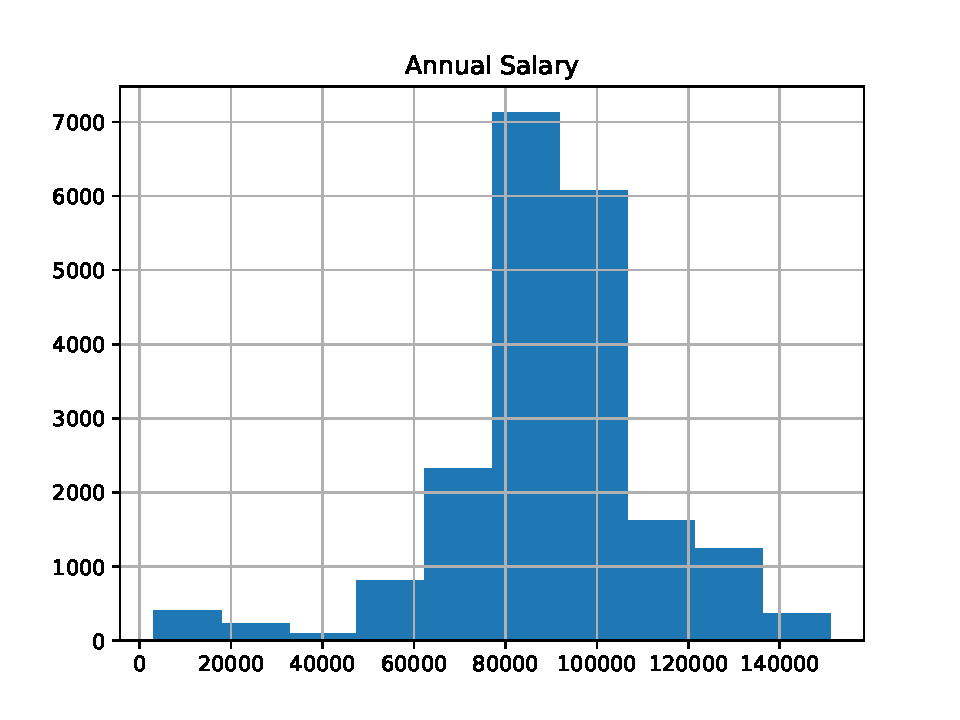
\includegraphics[width=0.75\textwidth]{figures/Chicago_annual_salary_distribution.pdf}
\caption{Distribution of the \textrm{Annual Salary} values for the Chicago dataset.}
\label{fig:chicago_fair-db1}
\end{figure}

The histogram of Figure~\ref{fig:chicago_fair-db2} shows instead the distribution of the annual salary of employees over their \textit{Gender} attribute, and it is particularly useful because it provides a preliminary visual representation of the discrepancy between the number of male and female employees belonging to the same bin, highlighting the fact that, although the amount of people earning more than \$90,000 is larger, there are many more women in the least profitable group.

\begin{figure}[h!]
\centering
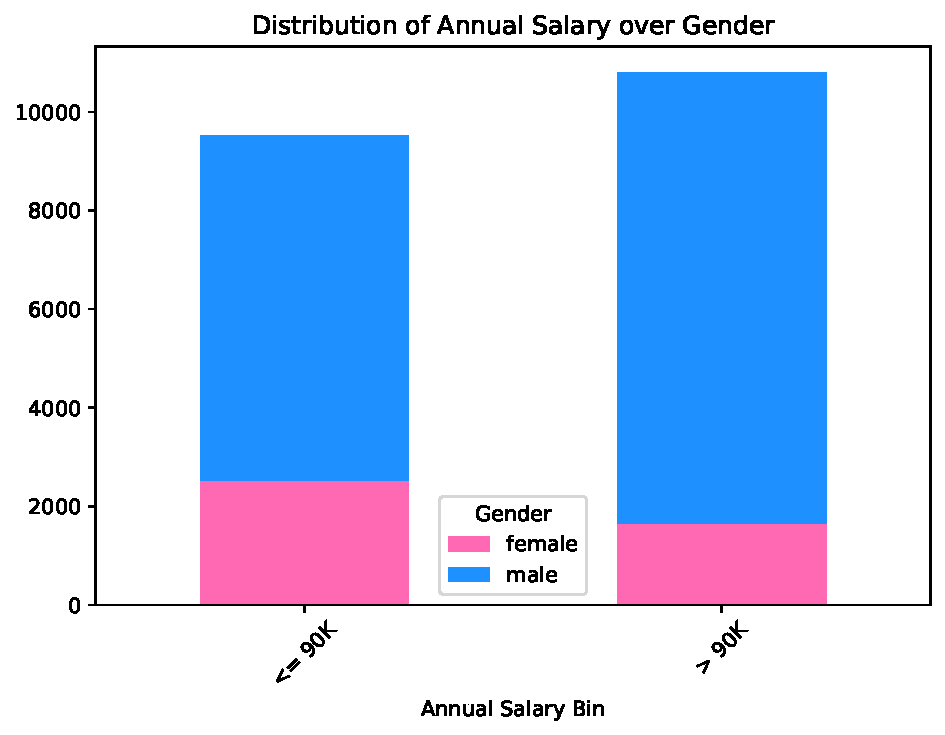
\includegraphics[width=0.75\textwidth]{figures/Chicago_2bins_annual_salary_over_gender.pdf}
\caption{Distribution of the \textrm{Annual Salary} values for the Chicago dataset (2 bins).}
\label{fig:chicago_fair-db2}
\end{figure}

Finally, we decided to plot the \textit{probability mass function (PMF)} and the \textit{cumulative distribution function (CDF)} of male and female employees, for each \textit{Annual Salary} value. For the laymen, PMF gives the probability that a discrete variable -- \textit{Annual Salary} in our case -- is exactly equal to a specific value; while CDF is the probability of the variable to be less than or equal to a specific value. The comparison between Figure~\ref{fig:chicago_fair-db3}(a) and Figure~\ref{fig:chicago_fair-db3}(b) shows, once again, that women are more likely than men to earn less, and specifically to have an income in the range of [0,~40K] dollars per year.

\begin{figure}[h!]
\centering
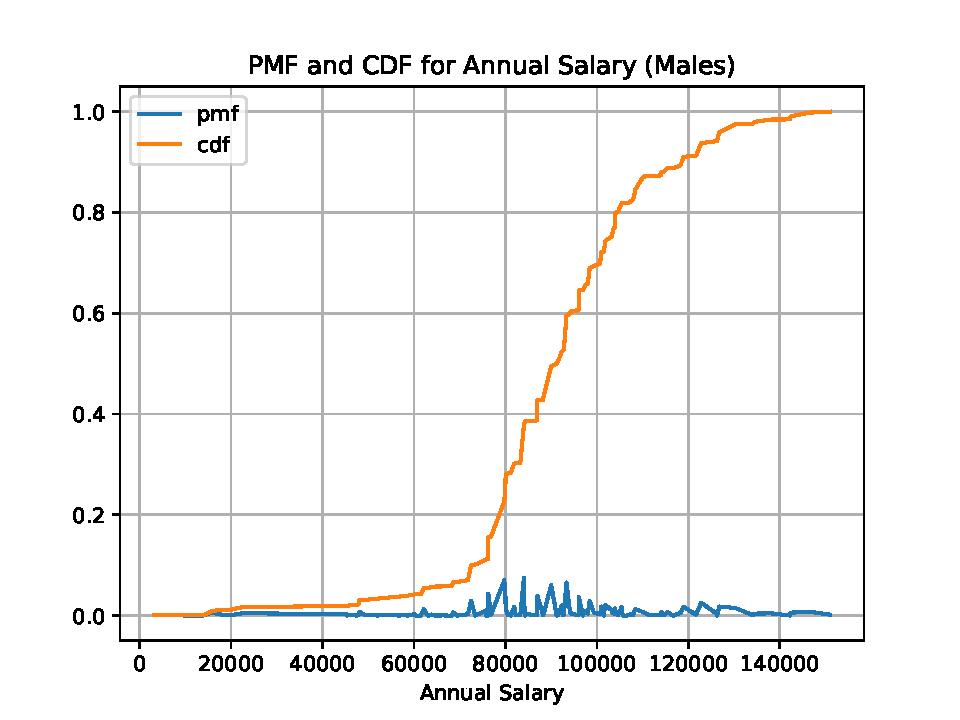
\includegraphics[width=0.75\textwidth]{figures/Chicago_pmf_cdf_annual_salary_males.pdf}
\caption*{(a)}
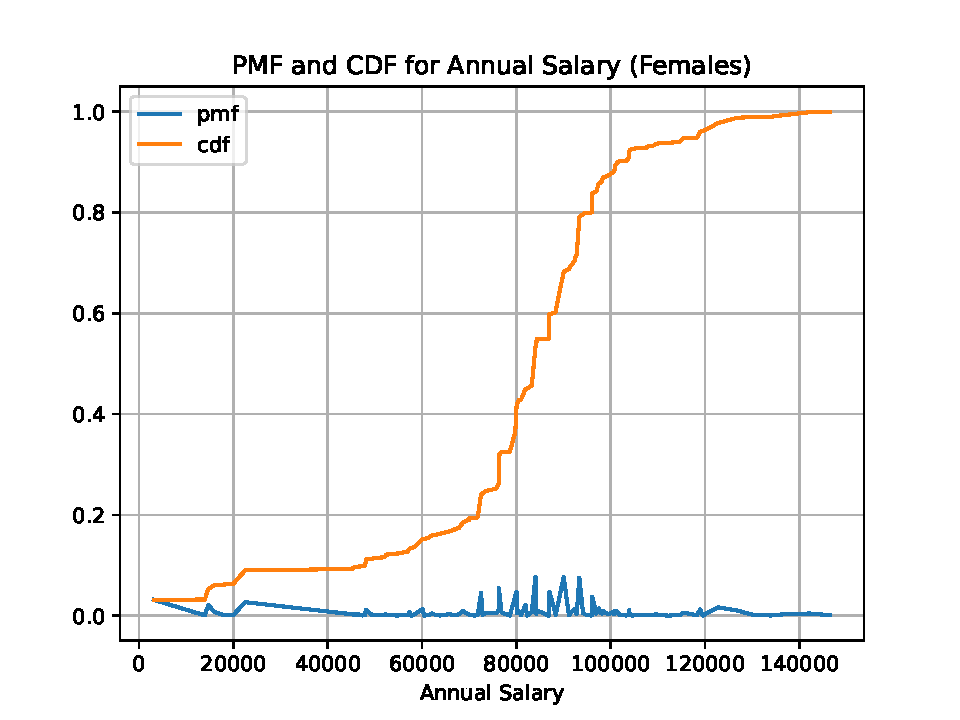
\includegraphics[width=0.75\textwidth]{figures/Chicago_pmf_cdf_annual_salary_females.pdf}
\caption*{(b)}
\caption{Probability mass function and cumulative distribution function of male (a) and female (b) employees, for each \textrm{Annual Salary} value of the Chicago dataset.}
\label{fig:chicago_fair-db3}
\end{figure}

Lastly, we performed a new \textbf{data reduction} operation by removing from the dataset the attributes \textit{Name} and \textit{Annual Salary}, not relevant anymore for our analysis, since the tool will make use of the \textit{Annual Salary Bin} variable.
\item \textbf{ACFD Discovery and filtering}: as specified in Section~\ref{section:fair-db}, this phase makes use of the \textit{ACFD Discovery} algorithm, presented in \cite{rammelaere2018revisiting}. The authors of the algorithm made available a compute capsule on Code Ocean\footnote{Available at: \url{https://codeocean.com/capsule/6146641/tree}.}, which works basically as a Web-based application, allowing the user to upload a CSV file (in our case, we exported and uploaded the modified Chicago dataset), run the algorithm and download the results in the form of a text file. Without going into too much detail, the algorithm is based on the notion of \textit{frequent itemsets}, that are itemsets in which elements have support greater than a minimum support threshold, and it takes as input \textit{minimum support}, \textit{minimum confidence} and \textit{maximum antecedent size} of the ACFD sought. The software also allows the choice of different algorithm implementations to be used to extract the dependencies but, as reported in the documentation, the default option FD-First-DFS-dfs is generally the fastest and there are no particular reasons, apart from performances, to choose one implementation over another.

Since our dataset does not contain a large amount of attributes, we decided to keep \textit{maximum~antecedent~size}~=~2 (meaning that at most 3 variables will appear in the LHS of the computed rules).
For what concerns the confidence, its value is computed as the ratio between the frequency of the dependency over the frequency of the LHS of the rule, and therefore a \textit{minimum~confidence}~=~0.8 seemed to be a reasonable threshold, since the lower the parameter, the more dependencies are generated at each round increasing the computational complexity and making more difficult the subsequent choice of the most interesting ACFDs.
Finally, we had to deal with the choice of a proper minimum support, which is quite a delicate operation: if it is too high the risk is to lose information about small groups, if it is too low there could be too many dependencies to analyze. We set \textit{minimum~support}~=~100, because it is a reasonably low number if compared to the total number of tuples in the dataset and to the average amount of tuples for each \textit{Job Title} value (\(\frac{20,309}{35} \simeq 580\)).

The text file generated by \textit{ACFD Discovery}, containing 714 rules, has to be filtered, since the dependencies detected could not involve any protected attribute and the target attribute, or there could be dependencies in which some attribute values are not specified. The authors of \cite{azzalini2021fair} did not use the compute capsule of \textit{ACFD Discovery}, and therefore were able to run the algorithm with an additional parameter, in order to discard the tuples not containing the target attribute and its value. We balanced the gap by importing the text file, parsing it in order to extract every rule, and doing the same filtering operation a posteriori of \textit{ACFD Discovery}. This operation resulted in a reduction in the number of dependencies from 714 to 145.

FAIR-DB then proceeds in filtering the rules by following 4 steps:
\begin{itemize}
\item[1.] For each dependency, LHS are separated from RHS, and from both antecedent and consequent every couple ``attribute - value'' is stored.
\item[2.] For each rule, every couple ``attribute - value'' is checked, and dependencies with missing values are discarded (being AFDs but not ACFDs).
\item[3.] A dictionary (that is, an unordered and indexed data structure similar to a list) of the remaining ACFDs is generated. It is made of two fields: `lhs' and `rhs', and each field contains a list of one or more couples ``attribute - value''.
\item[4.] Since each rule of the dictionary contains the target attribute but not necessarily any protected attribute, the dependencies are furtherly parsed in order to satisfy both the criteria.
\end{itemize}

For the Chicago dataset, the filtering operation resulted in a reduction in the number of dependencies from 145 to 49. For each rule, the metrics \textit{support}, \textit{confidence}, \textit{difference} and \textit{p-Difference}, already introduced in Section~\ref{section:evaluation_metrics} and Section~\ref{section:fair-db}, are computed, and the first occurrencies are displayed in the form of a table, as shown in Figure~\ref{fig:chicago_fair-db4}.

\begin{figure}[h!]
\centering
\noindent\rule{\linewidth}{0.4pt}\par
%\resizebox{\linewidth}{!}{%
\scalebox{.9}{\BVerbatimInput{figures/chicago_fair-db4.txt}}
\noindent\rule{\linewidth}{0.4pt}
\caption{First 5 filtered dependencies with their metrics for the Chicago dataset (2 bins). NaN (Not a Number) means that the p-Difference has not been computed for the specific rule, since the protected attribute is not in the antecedent.}
\label{fig:chicago_fair-db4}
\end{figure}

\item \textbf{ACFDs selection}: in this phase FAIR-DB selects, among the filtered rules, the most ``unethical'', by looking at the computed metrics. It is worth to briefly recap the meanings behind the measures:
\begin{itemize}
\item \textbf{Support}: it expresses the percentage of records in the dataset that verifies the dependency -- the higher the value, the more tuples are involved.
\item \textbf{Confidence}: it shows how frequently the dependency is verified knowing that the antecedent is verified -- the higher the value, the less approximate is the dependency.
\item \textbf{Difference}: it indicates how much a dependency is ``unethical'' -- the higher the value, the more unfair is the dependency.
\item \textbf{p-Difference}: it indicates how much the dependency shows bias paying attention to the specific value of a protected attribute -- the higher the value, the more the rule is discriminatory with respect to the specific protected attribute value.
\end{itemize}

The selection of the most relevant rules takes place automatically, since the algorithm keeps only the dependencies with a difference parameter value higher than a minimum threshold imposed by the user. We decided to set \textit{minimum~difference}~=~0.02, in order to keep the majority of the unfair dependencies. This operation resulted in a reduction in the number of dependencies from 49 to 10.

After that, the algorithm performs what the authors call \textbf{ACFDs completion}. Given the selected ACFDs, the framework computes all the possible combinations for each rule over the protected attributes and the target attribute (performing a Cartesian product between the attributes values). Taking as an example ACFD n.0 of Figure~\ref{fig:chicago_fair-db4}: \[\mathit{Annual Salary Bin} = \mlq > 90K \mrq \rightarrow \mathit{Gender} = \mlq \mathrm{male} \mrq\] we identify \textit{Annual Salary Bin} as target attribute, whose possible values are \(\leq\)~90K and >~90K, and \textit{Gender} as protected attribute, whose possible values are male and female. Therefore, the possible combinations for the rule are:
\begingroup\belowdisplayskip=\belowdisplayshortskip
\[\mathit{Annual Salary Bin} = \mlq > 90K \mrq \rightarrow \mathit{Gender} = \mlq \mathrm{male} \mrq\]\endgroup
\[\mathit{Annual Salary Bin} = \mlq \leq 90K \mrq \rightarrow \mathit{Gender} = \mlq \mathrm{male} \mrq\]
\[\mathit{Annual Salary Bin} = \mlq > 90K \mrq \rightarrow \mathit{Gender} = \mlq \mathrm{female} \mrq\]
\[\mathit{Annual Salary Bin} = \mlq \leq 90K \mrq \rightarrow \mathit{Gender} = \mlq \mathrm{female} \mrq\]
For each newly generated dependency, the evaluation metrics are computed, and a new automatic selection is performed, by keeping the rules with difference greater than the respective minimum threshold. ACFDs completion basically allows the user to study all the domain of the protected attributes and of the target class, and the combination computation brings to the surface also small groups that could not be studied otherwise. This operation, for the Chicago dataset, generated 36 dependencies (including the original 10), of which 18 with a difference above the threshold.
\item \textbf{ACFDs ranking}: the dependencies are ranked in descending order of support, difference, or mean, according to the user's choice. As already mentioned in Section~\ref{section:fair-db}, the support option highlights the pervasiveness of the rules, the difference highlights their unethical aspect, and the mean represents the best trade-off between difference and support. Because of that, we decided to adopt the mean as ordering criterion. The resulting table is finally printed, and Figure~\ref{fig:chicago_fair-db5} shows the first 5 dependencies (the others are displayed to the user but are omitted here for the sake of brevity).

\begin{figure}[h!]
\centering
\noindent\rule{\linewidth}{0.4pt}\par
%\resizebox{\linewidth}{!}{%
\scalebox{.9}{\BVerbatimInput{figures/chicago_fair-db5.txt}}
\noindent\rule{\linewidth}{0.4pt}
\caption{First 5 selected and ranked dependencies with their metrics for the Chicago dataset (2 bins).}
\label{fig:chicago_fair-db5}
\end{figure}

\item \textbf{ACFDs user selection and scoring}: this last phase requires interaction from the user, who has to select \(N\) interesting dependencies among the ones previously ranked. The system then computes a final scoring outline based on 3 measures:
\begin{itemize}
\item \textbf{Cumulative support}: percentage of tuples of the dataset involved by the selected ACFDs -- the higher the value, the more tuples are involved.
\item \textbf{Difference mean}: arithmetic mean of all the `Difference' columns of the selected ACFDs. It indicates how much the dataset is ethical according to the chosen rules -- the higher the value, the more unfair is the dataset.
\item \textbf{Protected attribute difference mean}: for each protected attribute, arithmetic mean of the p-Difference measure over all the selected ACFDs. It indicates how much the dataset is ethical over the protected attribute according to the chosen rules -- the higher the value, the more the dataset is discriminatory with respect to the specific protected attribute.
\end{itemize}

For our research, we selected all the dependencies in which the target attribute appears in the RHS of the rule (\(N\) = 6 out of 18). The chosen ACFDs, together with the final scores, are displayed in Figure~\ref{fig:chicago_fair-db6}.

\begin{figure}[h!]
\centering
\noindent\rule{\linewidth}{0.4pt}\par
%\resizebox{\linewidth}{!}{%
\scalebox{.9}{\BVerbatimInput{figures/chicago_fair-db6.txt}}
\noindent\rule{\linewidth}{0.4pt}
\caption{Final selected rules and scores for the Chicago dataset (2 bins).}
\label{fig:chicago_fair-db6}
\end{figure}
\end{itemize}

Among the chosen dependencies, we can detect a correspondency between rule 7 and rule 4: women paid on a hourly basis tend to earn less than \$90K, while men paid on a hourly basis tend to earn more than \$90K. These rules are the ones with the higher support (respectively 0.03 and 0.07), and rule 7 is the one with the highest difference value (0.24).
Even though the support is very low -- and therefore not many tuples out of the total are involved -- it is important to point out that rules 27 and 24 highlight a discriminatory behavior in the subgroup of the AVIATION department, while rules 29 and 30 show that, for what concerns the OEMC department, men seem to be less paid than women.

As for the scoring measures, a cumulative support of 0.114 means that the 11.4\% of the dataset is ``problematic'' (2,310 tuples out of 20,309), while difference mean and gender difference mean (equal because in our dataset \textit{Gender} is the only protected attribute) have a value of 0.094 because of the gap between the difference metric values of the selected ACFDs (above 0.1 for rule 27, above 2 for rule 7, below 1 for the other rules).

To conclude, we can say that the dataset seem to be quite fair with respect to the group fairness criterion, that is the one on which the tool is based, but more than 10\% of the tuples show some bias. Furthermore, the representation problem is not taken into account, and therefore the tendency of women to be employed in less profitable jobs than men, displayed in Figure~\ref{fig:chicago_fair-db2} and Figure~\ref{fig:chicago_fair-db3} is ignored.


\subsection{Ranking Facts}
As specified in Section~\ref{section:ranking_facts}, Ranking Facts is primarily meant to be a Web-based application with the aim of discovering fairness in a dataset by making use of ranking and providing to the user a collection of visual widgets. However, because of the size of our dataset, we could not use the tool in the form of Web-based application, and we therefore opted for the notebook version.

Before importing the dataset, we had to deal with a further \textbf{data transformation} process, in which we converted our categorical attributes (\textit{Status}, \textit{Job Title}, \textit{Department}, \textit{Salary or Hourly}) into numerical ones, since the tool can perform ranking only over them. A value of F for the \textit{Status} attribute was therefore converted to 1, while P was converted to 0. The same holds for \textit{Salary or Hourly} (Salary = 1, Hourly = 0), while for \textit{Job Title} and \textit{Department} numbers from 0 to 35 and from 0 to 20 respectively substited the original categorical values.

Once imported the dataset, the tool initially plots the distribution of some attributes specified by the user (in our case, we decided to plot the distributions of the \textit{Annual Salary} and \textit{Gender} values). While the related distribution graphs are not particularly meaningful, the heatmap generated subsequently provides us some preliminary information about the attributes correlations. As Figure~\ref{fig:chicago_rankingfacts1} shows, there seem to be a significant correlation between \textit{Job Title} and \textit{Department}, but mostly important between \textit{Status} and \textit{Annual Salary}, \textit{Status} and \textit{Salary or Hourly}, and finally \textit{Annual Salary} and \textit{Salary or Hourly}, highlighting the fact that hourly paid and part-time employees earn generally less than salary paid and full-time employees, and most of the part-time workers are also being paid on a hourly basis.

\begin{figure}[h!]
\centering
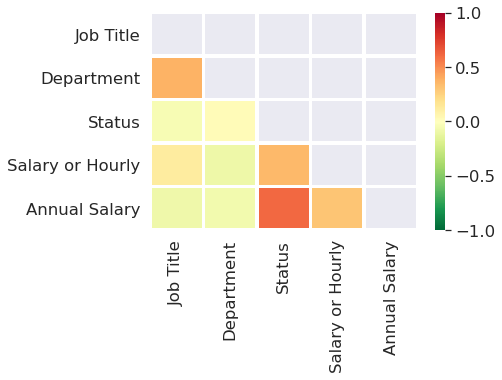
\includegraphics[width=0.75\textwidth]{figures/chicago_rankingfacts1.png}
\caption{Heatmap showing attributes correlations for the Chicago dataset.}
\label{fig:chicago_rankingfacts1}
\end{figure}

The tool then requires the user to specify some attributes to be used for the ranking, together with their weights. The reference formula is: \[f(x) = w_1 * \mathit{Attribute}_1(x) + \ldots + w_n * \mathit{Attribute}_n(x)\]
In our case, the attributes used are \textit{Job Title}, \textit{Department}, \textit{Status}, and \textit{Salary or Hourly}, because they are numerical and none of them is a protected or a target variable. By following the examples provided by the authors of the tool, we decided to set the weights all equal to 1, giving the same importance to each attribute.

By following the widgets descriptions list provided in Section~\ref{section:ranking_facts}, we will now summarize our results.
\begin{itemize}
\item \textbf{Recipe} and \textbf{Ingredients}: the notebook version of the tool unfortunately does not provide any visual representation. As for the recipe, a couple of summary tables display some statistical measures (median, mean, minimum and maximum value) for the 4 attributes used in the ranking, respectively for the top-10 one and overall. These tables are not particularly useful, and neither are the information related to the ingredients, which tell us that the importance of each attribute used for the ranking is effectively equal to 1.
\item \textbf{Stability}: this parameter explains wheter the ranking methodology is robust on the specific dataset in use. Since an unstable ranking is one where slight changes to the data or to the methodology could lead to a significant change in the output, the label reports a stability score, as a single number that indicates the extent of the change required for the ranking to change. The stability of the ranking is quantified as the slope of the line that is fit to the score distribution, at the top-10 and overall. A score distribution is unstable if scores of items in adjacent ranks are close to each other (\(|\mathit{slope}| \leq 0.25\)), and so a very small change in scores will lead to a change in the ranking. The ranking used to analyze the Chicago dataset resulted to be unstable both at top-10 (stability at 0.23) and overall (stability at 0.0), and the score distribution is displayed in Figure~\ref{fig:chicago_rankingfacts2}.

\begin{figure}[h!]
\centering
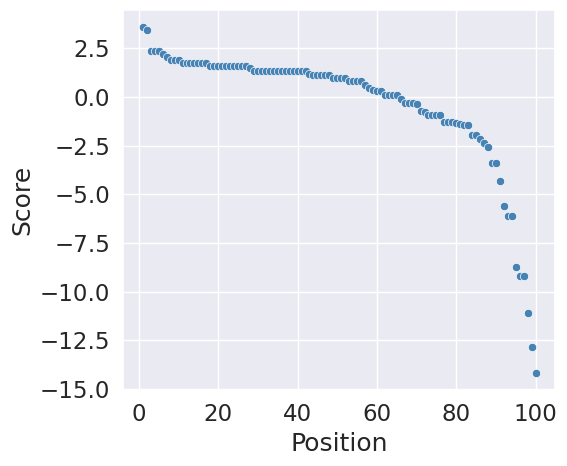
\includegraphics[width=0.75\textwidth]{figures/chicago_rankingfacts2.png}
\caption{Score distribution of the ranking for the Chicago dataset.}
\label{fig:chicago_rankingfacts2}
\end{figure}

\item \textbf{Fairness}: it quantifies whether the ranked output exhibits statistical parity (group fairness) with respect to one or more protected attributes. The fairness measures adopted are all statistical tests in which the null hypothesis is that the ranking process is fair for the protected group, and whether a result is fair is determined by the computed \(p\)-value (a ranking is considered unfair when the \(p\)-value of the corresponding statistical test falls below 0.05).
\begin{itemize}
\item \textbf{FA*IR}: the ranking resulted to be \textit{fair for males}, with an approximate \(p\)-value of 0.94, and \textit{fair for females}, with an approximate \(p\)-value of 0.23.
\item \textbf{Proportion}: the ranking resulted to be \textit{fair for males}, with an approximate \(p\)-value of 0.94, and \textit{fair for females}, with an approximate \(p\)-value of 0.35.
\item \textbf{Pairwise}: the ranking resulted to be \textit{unfair for males}, with an approximate \(p\)-value of 0.0, and \textit{fair for females}, with an approximate \(p\)-value of 0.99.
\end{itemize}
The results seem to be oriented towards a fair dataset, however the pairwise measure reported an exceptional bias in favor of women, which is quite peculiar because with the previously adopted tools the trend was towards fairness but with a slight tendency in favor of men.
\item \textbf{Diversity}: it shows diversity with respect to a set of demographic categories of individuals, or a set of categorical attributes of other kinds of items, by displaying the proportion of each category in the top-10 ranked list and overall. Figure~\ref{fig:chicago_rankingfacts3} shows the predominancy of the male group over the female one, highlighting again a problem of gender representation.

\begin{figure}[h!]
\centering
\begin{minipage}{0.45\textwidth}
\centering
\includegraphics[width=\textwidth]{figures/Chicago_rankingfacts3a.png}
\caption*{(a)}
\end{minipage}
\begin{minipage}{0.45\textwidth}
\centering
\includegraphics[width=\textwidth]{figures/Chicago_rankingfacts3b.png}
\caption*{(b)}
\end{minipage}
\caption{\textrm{Gender} diversity widget for the top-10 (a) and overall (b) rankings of the Chicago dataset.}
\label{fig:chicago_rankingfacts3}
\end{figure}

\end{itemize}


\newpage
\section{Case Study 2: San Francisco}
\subsection{Data Preprocessing}
\subsection{The ``Glassdoor Method''}
\subsection{FAIR-DB}
\subsection{Ranking Facts}


\section{Other Design Choices}


\iffalse

\note{Figures and tables}{You are an engineer, and using figures (illustrations) and tables to better convey your ideas should be an obvious practice you should have learned throughout your university career. If not, it's time now. Use illustrations, screen shots, sketches, and so on to help the reader understand. Use tables to summarize complex text (for example, a profound analysis of the state of the art) or to format data in a readable fashion. Each time you use a figure or table, you must also (i) complement it with a so-called caption (a text right underneath or above it) to give it a title and a description and (ii) reference it from within the main text (never just place a figure somewhere without talking about it). If you use Latex, check your Latex documentation for how to use captions and references.}

\fi
